%%%%%%%%%%%%%%%%%%%%%%%%%%%%%%%%%%%%%%%%%
% University Assignment Title Page 
% LaTeX Template
% Version 1.0 (27/12/12)
%
% This template has been downloaded from:
% http://www.LaTeXTemplates.com
%
% Original author:
% WikiBooks (http://en.wikibooks.org/wiki/LaTeX/Title_Creation)
%
% License:
% CC BY-NC-SA 3.0 (http://creativecommons.org/licenses/by-nc-sa/3.0/)
% 
% Instructions for using this template:
% This title page is capable of being compiled as is. This is not useful for 
% including it in another document. To do this, you have two options: 
%
% 1) Copy/paste everything between \begin{document} and \end{document} 
% starting at \begin{titlepage} and paste this into another LaTeX file where you 
% want your title page.
% OR
% 2) Remove everything outside the \begin{titlepage} and \end{titlepage} and 
% move this file to the same directory as the LaTeX file you wish to add it to. 
% Then add \input{./title_page_1.tex} to your LaTeX file where you want your
% title page.
%
%%%%%%%%%%%%%%%%%%%%%%%%%%%%%%%%%%%%%%%%%
%\title{Title page with logo}
%----------------------------------------------------------------------------------------
%	PACKAGES AND OTHER DOCUMENT CONFIGURATIONS
%----------------------------------------------------------------------------------------

\documentclass[12pt]{article}
\usepackage[english]{babel}
\usepackage[utf8x]{inputenc}
\usepackage{amsmath}
\usepackage{graphicx}
\usepackage[colorinlistoftodos]{todonotes}

\begin{document}

\begin{titlepage}

\newcommand{\HRule}{\rule{\linewidth}{0.5mm}} % Defines a new command for the horizontal lines, change thickness here

\center % Center everything on the page
 
%----------------------------------------------------------------------------------------
%	HEADING SECTIONS
%----------------------------------------------------------------------------------------

\textsc{\LARGE Università degli studi di Milano-Bicocca}\\[1cm] % Name of your university/college
\textsc{\Large Advanced Machine Learning }\\[0.3cm] % Major heading such as course name
\textsc{\large Final Project}\\[0.1cm] % Minor heading such as course title

%----------------------------------------------------------------------------------------
%	TITLE SECTION
%----------------------------------------------------------------------------------------

\HRule \\[0.4cm]
{ \huge \bfseries Flowers recognition}\\[0.4cm] % Title of your document
\HRule \\[1.5cm]
 
%----------------------------------------------------------------------------------------
%	AUTHOR SECTION
%----------------------------------------------------------------------------------------

\large
\emph{Author:}\\
David Bertoldi - 735213 - d.bertoldi@campus.unimib.it \\[1cm]  % Your name


% If you don't want a supervisor, uncomment the two lines below and remove the section above
%\Large \emph{Author:}\\
%John \textsc{Smith}\\[3cm] % Your name

%----------------------------------------------------------------------------------------
%	DATE SECTION
%----------------------------------------------------------------------------------------

{\large \today}\\[2cm] % Date, change the \today to a set date if you want to be precise

%----------------------------------------------------------------------------------------
%	LOGO SECTION
%----------------------------------------------------------------------------------------


\includegraphics{logo.png}\\[1cm] % Include a department/university logo - this will require the graphicx package
 
%----------------------------------------------------------------------------------------

\vfill % Fill the rest of the page with whitespace

\end{titlepage}


\begin{abstract}
The ABSTRACT is not a part of the body of the report itself. Rather, the abstract is a brief summary of the report contents that is often separately circulated so potential readers can decide whether to read the report. The abstract should very concisely summarize the whole report: why it was written, what was discovered or developed, and what is claimed to be the significance of the effort. The abstract does not include figures or tables, and only the most significant numerical values or results should be given.
\end{abstract}

\section{Introduction}


The aim of this work is to build a machine learning model able to learn from a small knowledge base and to classify similar images but belonging to different classes.
The main issue to overcome was the high chance that the model could overfit and fail to classify unseen samples. The strategy adopted was to find the model exploiting transfer learning the best and tryed to freeze the model such that it maintained similar performances. \par
This document describes the research on trained models, hyperparameters and generalization techniques that allowed the model to operate on a large variety of images. 






\section{Datasets}
The dataset used is the \textit{102 Category Flower Dataset} \cite{Nilsback08} created by the researchers of the \textit{Visual Geometry Group} of \textit{Oxford}. The dataset is composed of $8\,189$ RGB images of variable size, each image contains one or more flowers on a neutral background and is labeled with a single category extracted from a set of $102$ possible categories. The original dataset also contains the flowers segmented from the background (Figure \ref{fig_dataset}); these images can be used for example as further input for the neural network. In this work they were not used in order to force the model to be more elastic with respect to the background of the images. \par
The subdivision of the dataset defined in the original publication has been maintained, in particular there are $1\,020$ images in the training set, $1\,020$ images in the validation set and $6\,149$ images in the test set.

\begin{figure}[ht!]
\centering  
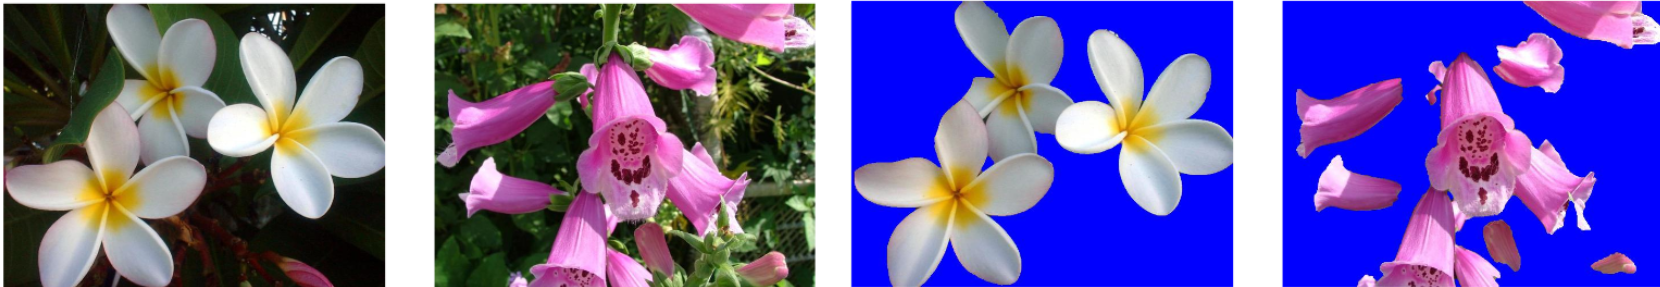
\includegraphics[width=1.0\textwidth]{images/dataset.png} 
\caption{Training images and their segmentation}
\label{fig_dataset}
\end{figure}

Each category is represented by $10$ images in the training set and validation set, while the proportion of images for each category varies in the test set.
The difficulty of operating on a dataset of this type is evident: the number of images for training is limited while the test set is larger. \par
Another peculiarity of the dataset is the presence of similar images belonging to different categories.





















\section{The Methodological Approach}

In order to classify images correctly two types of experiment were taken in accont: the first one aimed to find the best CNN\footnote{Convolutional Neural Network} architectures in 
literature that could fit the available hardware (see Section \ref{sec:tech}) and the second tried to find a good trade-off between number of trainable layers and accuracy by freezing the layers' weights during training. \par
All the proposed architecture were pre-trained on \textit{ImageNet} and used as feature extractors for a new classifier that operates over 102 classes.

\subsection{Technology and implementation}\label{sec:tech}
The hardware used for this work was composed by a GPU NVIDIA 2070 SUPER with 8GB of VRAM, a CPU Intel i7-9700K $3.6$GHz and $32$GB of RAM. \par
The libraries used were \textit{Keras}, based on \textit{Tensorflow}, for learning and preprocessing, \textit{sklearn} for metrics and \textit{numpy}  for generic calculation.
\todo{Github}

\subsection{Preprocessing and Data Augmentation}
Before proceeding with the description of the experiments, there was a preliminar implicit objective: how to overcome the scarcity of training data.\par
In order to raise the number of samples it was used \texttt{ImageDataGenerator} from \textit{Keras}. This allowed to virtually loop infinitely on the images during the training and most importantly to transform each of these images by applying none, one or more of the following transformations:
\begin{itemize}
\item{Horizontal flipping}
\item{Rotation of angle $\alpha \in [-20^{\circ}, 20^{\circ}]$}
\item{Shift of brightness $\gamma \in [0.7, 1.3]$}
\item{Zoom  $\zeta \in [0.8, 1.2]$}
\end{itemize}
Additionally every image is transformed with the original preprocessing function used for the training of the original architecture on \textit{ImageNet}.\todo{preprocessing}



\subsection{Hyper-parameters}
To train the perceptron on the extracted features it was decided to use the SGD with momentum $\beta = 0.9$ or Adam with $\beta_1 = 0.9$ and $\beta_2 = 0.999$, with dimension of
batch equal to $64$ and momentum equal to 0.9. 
Since the task is a classification over multiple categories the chosen objective function to minimize was \emph{categorical cross-entropy}. \par

The learning rate $\eta$ is calculated according to the algorithm described in \emph{"Cyclical Learning Rates for Training Neural
Networks”}. This algorithm made $\eta$ fluctuate forward and
back in a fixed interval $I$ at each iteration during the training phase;
this strategy had a dual purpose: to reduce the bias introduced by choosing a non-optimal $\eta$ during the design phase and to help the optimizer to escape from saddle points or 
from local minima that could block its correct covergence.\par

To calculate the aforementioned interval $I$ of values the authors described the following algorithm:
\begin{enumerate}
\item{Choose an interval $J$ on which to make vary $\eta$. For this work $I = [10^{-10}, 10^{-1}]$ was used} 
\item{Train the model for few epochs (\textit{e.g.} 10) starting with the smallest ${\eta}' \in J$. At the end of each epoch exponentially increase ${\eta}'$}
\item{Stop the training when $\eta$ reached the upper bound of $J$}
\item{Plot the fluctuation of the loss function realtive to ${\eta}'$}
\end{enumerate}
As an example, the algorithm generated the plot in Figure \ref{fig:lr} for optimizer Adam and the architecture described in section \todo{section}. 
\begin{figure}[ht]
\centering
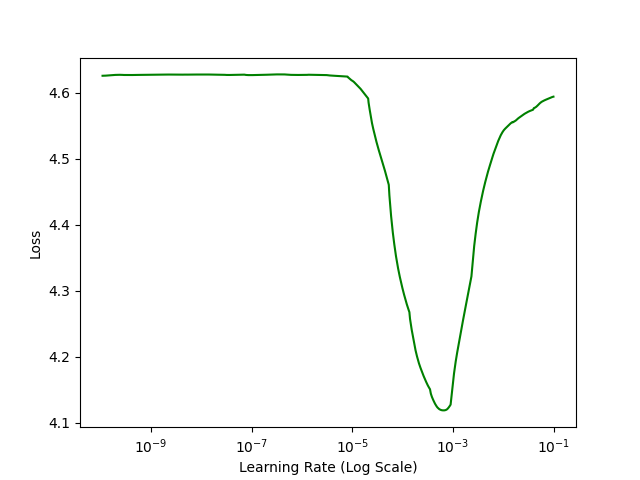
\includegraphics[width=0.8\textwidth]{images/lr_adam.png} 
\caption{Output of the learning rate finder algorithm. $I=[10^{-5}, 10^{-3}]$ is the optimal solution}
\label{fig:lr}
\end{figure}

The graph show how the network begins to learn starting from $\eta \simeq 10^{-5}$ and diverges once $\eta$ exceeded $\sim10^{-3}$; these two values were used as extremes of $I$ for the cyclical learning rate algorithm on this particular architecture.\par
The drawback of this strategy is that it added two additional hyper-parameters: the step size $s$, that determined the number of iterations required to go from the minimum $\eta$ to the maximum, and the cyclical learning rate schedule, that defined the way $\eta$ is modified. \par

Figure \ref{fig:triangular} shows the two schedules used for this work: \emph{Triangular} and \emph{Triangular2};
the difference between the two is that the second method halves the upper bound of $I$ at each cycle completion.
\begin{figure}[ht!]
\centering
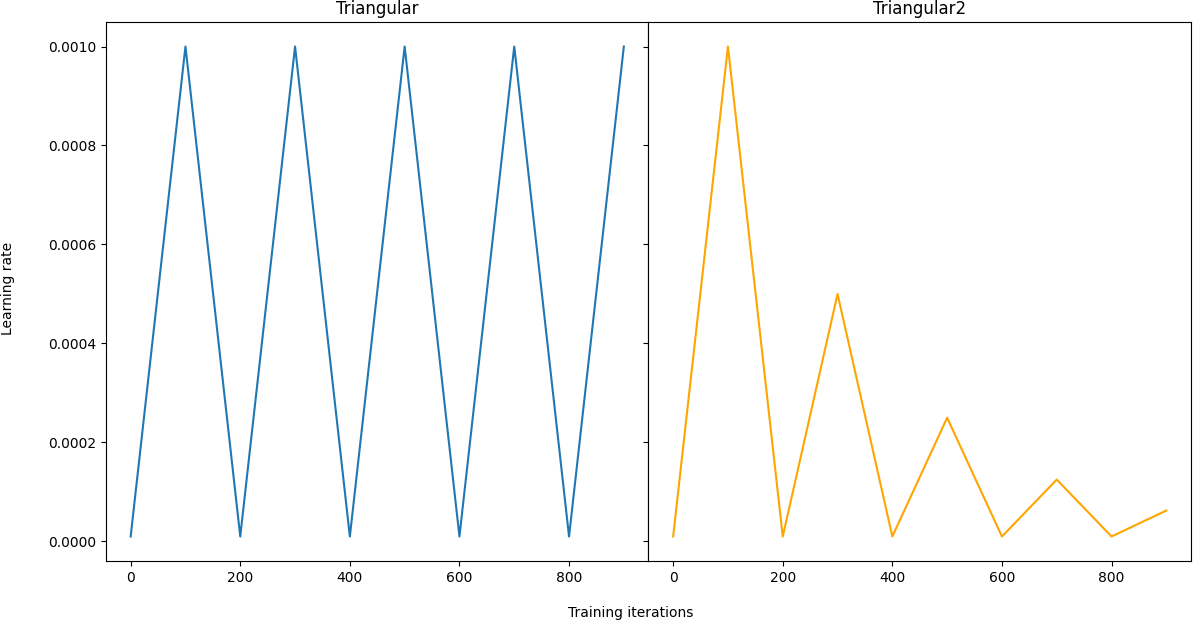
\includegraphics[width=1\textwidth]{images/triangular.png} 
\caption{Plot of the learning rate with \emph{Triangular} and \emph{Triangular2} methods}
\label{fig:triangular}
\end{figure}








\subsection{Experiment 1: Choice of the architecture}
The first experiment aimed to find the architecture that could achieve the best accuracy on the test set. This work tested \textit{ResNet18}, \textit{InceptionV3} and 
\textit{EfficientNetB4}. All of them presented diffent peculiarities and could be used for training with the available hardware. \par
Since the training on \textit{ImageNet} of the networks is not sufficient to use them as feature extractors, the entire networks were fine-tuned in order to update their weights and to fit better the task.
\begin{figure}[ht!]
\centering
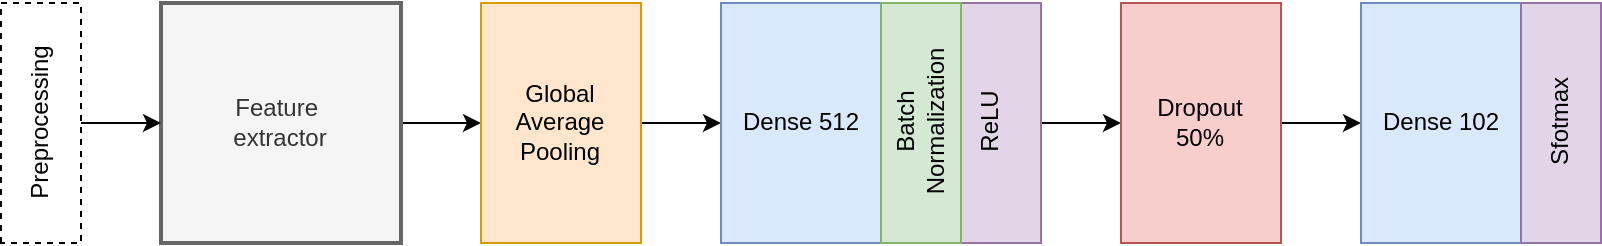
\includegraphics[width=1\textwidth]{images/architecture.png} 
\caption{Plot of the learning rate with \emph{Triangular} and \emph{Triangular2} methods}
\label{fig:architecture}
\end{figure}
To each networks the original classification layers were removed and substituted with a new classifier composed by the following layers:
\begin{enumerate}
\item{\textbf{Global Average Pooling}: instead of using a Flatten layer that could raise the risk of overfitting and forced the use of Dropout, this layer applied average pooling on the spatial dimensions until each spatial dimension is one, and leaves other dimensions unchanged. It added 0 new parameters to the model} 
\item{\textbf{Dense 512}: a dense layer with a \textbf{Batch Normalization} before the activation function (ReLU). This helped to avoid vanishing/exploding gradients when training the model. It added $512 \cdot (n+1) + 4\cdot512 = 512n + 2\,560$ parameters}
\item{\textbf{Dropout} as regularization technique for reducing overfitting during training, with a drop rate $\rho=0.5$. It added 0 new parameters to the model}
\item{\textbf{Dense 102}: a dense layer that used softmax as activation function. It added  $102 \cdot (512+1) = 52\,326$ new parameters}
\end{enumerate}

The total number of parameters added to the original feature extractor is $512n + 54\,886$, where $n$ is the dimensionality of the last layer of the feature extractor.\par
The strategy adopted for training is the same for all the three networks: each network is trained with 3 different step sizes, two different optimizers and 2 different learning rate schedulers. So each network is trained 12 times in order to find the best configuration. For this phase it was implemented the Early Stopping technique in order to prevent overfit and to speed up the training by stopping prematurely the process. This strategy monitored the validation accuracy and stopped everytime a model could not improve by $1\%$ in the last $10$ epochs.



\subsubsection{Fine-tuning of ResNet-18}\label{sec:resnet18}
ResNet-18 is a convolutional neural network that is 18 layers deep and accepts images of input size of $224 \times 224$. It is a residual network, that is it implements skip connections to help to address the problem of vanishing  gradients. \par
The preprocessing function applied on the images converted them from RGB to BGR, then each color channel was zero-centered with respect to the \textit{ImageNet} dataset, without scaling. \par
From the output of the \textit{LRF} algorithm the learning rate was varied in the interval $[10^{-5}, 10^{-3}]$ for SGD and $[10^{-6}, 10^{-4}]$ for Adam.


\subsubsection{Fine-tuning of InceptionV3}\label{sec:inceptionv3}
InceptionV3 is a convolutional neural network that is 42 layers deep and accepts images of input size of $299 \times 299$. This architecture factorizes the larger convolutions  into smaller ones and and uses an auxiliary classifer to propagate label information lower down the network.
 \par
The preprocessing function applied on the images scaled their pixels between -1 and 1, sample-wise. \par
From the output of the \textit{LRF} algorithm the learning rate was varied in the interval $[10^{-5}, 10^{-2}]$ for SGD and $[10^{-3}, 10^{-3}]$ for Adam.


\subsubsection{Fine-tuning of EfficientNetB4}\label{sec:efficientb4}
EfficientNetB4 is a convolutional neural network that is 237 layers deep and accepts images of input size of $224 \times 224$. 
This type of architecture was built using automatic search and scaling techniques
aimed to simultaneously maximize the accuracy of the network and the number of operations per second. \par
There was no need to apply the ad-hoc preprocessing function because it was embedded in the Keras implementation. \par
From the output of the \textit{LRF} algorithm the learning rate was varied in the interval $[10^{-5}, 10^{-3}]$ fboth or SGD and Adam.


\subsection{Evaluation of the training}
To verify the quality of the training two techniques were applied: \textit{grad-CAM} and \textit{Saliency Map}. Confusion matrices as well helped indentifying
issues in the first stages of the implementation.

\subsubsection{grad-CAM}
\textit{grad-CAM} uses the gradient of the last convolutional layer so that the spatial information are preserved. An heatmap is displayed over the original image
that shows the main component identified by the network.

\begin{figure}[ht!]
\centering
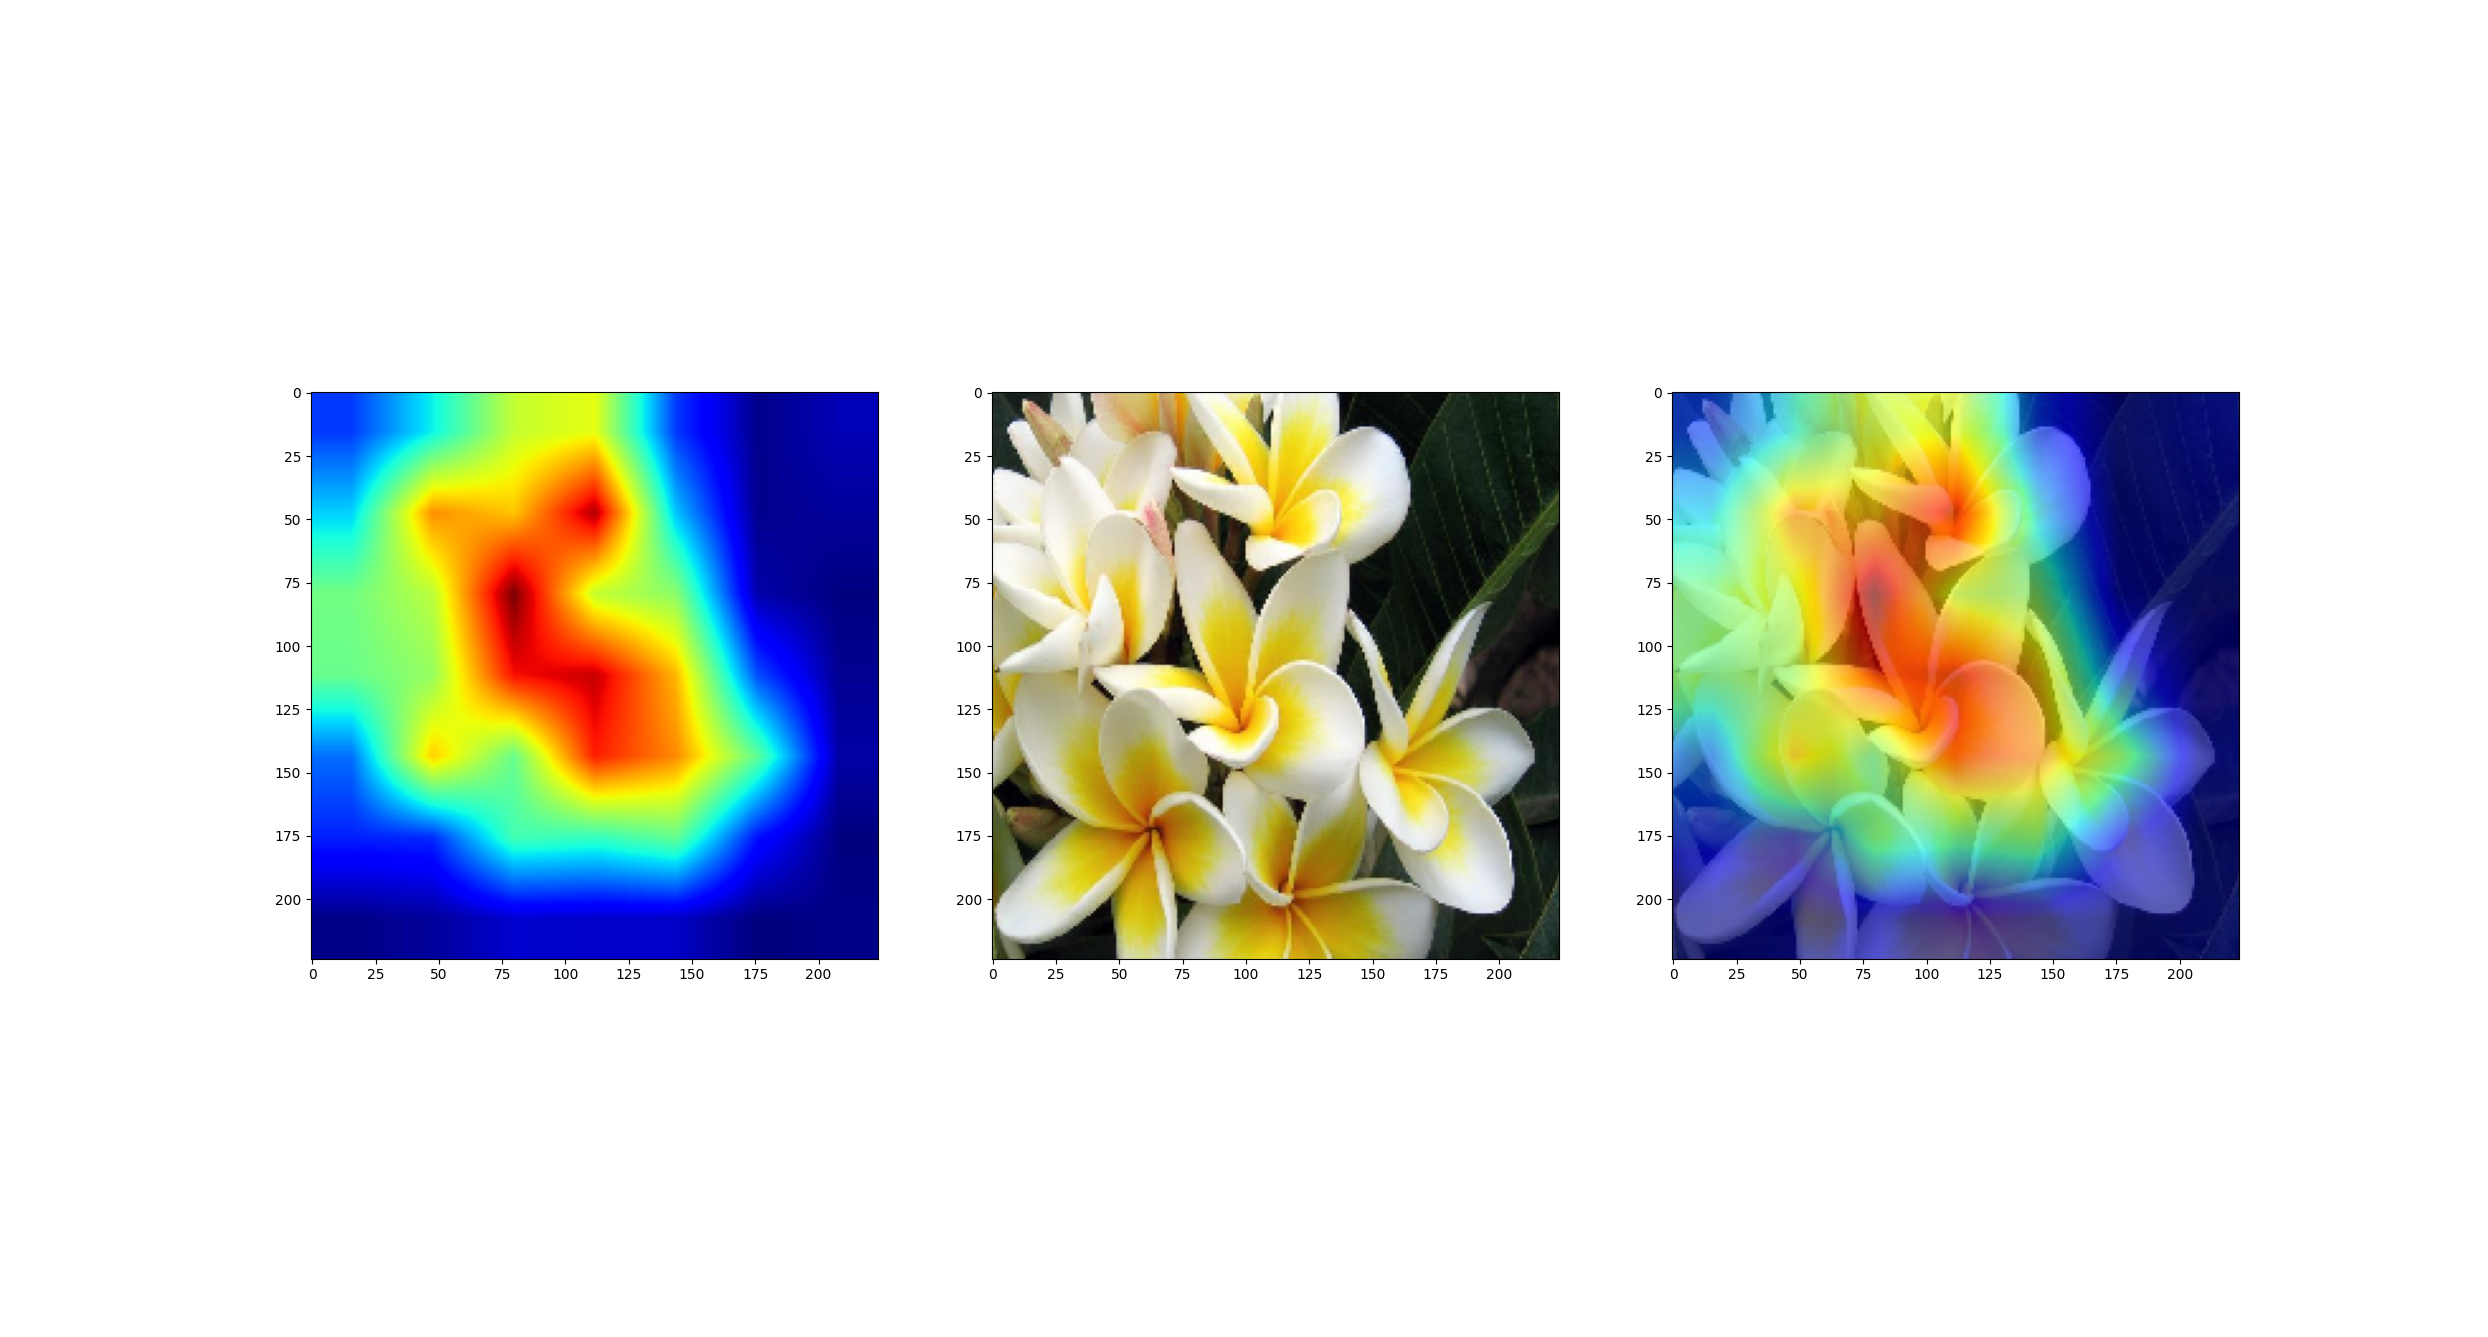
\includegraphics[width=1\textwidth]{images/grad_multi.png} 
\caption{\textit{grad-CAM} of multiple flowers}
\label{fig:grad_multi}
\end{figure}

Figure \ref{fig:grad_multi} demonstrates that the model could distinguish the flowers from the background and that the background is not an important 
feature to be learned.


\subsubsection{Saliency Map}
Like the \textit{grad-CAM}, \textit{Saliency Maps} analyze a specific layer of the model, but in this case it is a classification layer. It shows the gradients of
an image with respect with the label. The map indicates the points that affected more the correct classification of the image.
\begin{figure}[ht!]
\centering
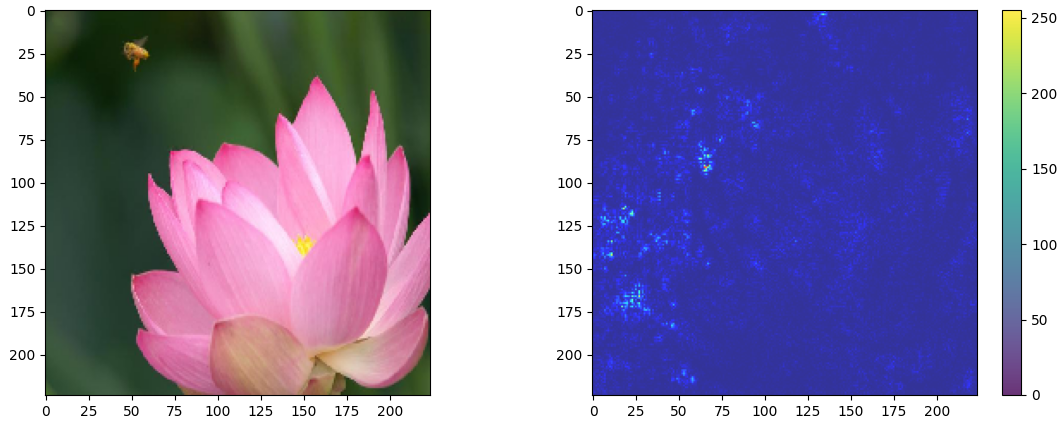
\includegraphics[width=1\textwidth]{images/sal_bee.png} 
\caption{\textit{Saliency Map} of a flower flown over by a bee}
\label{fig:sal_bee}
\end{figure}
For example Figure \ref{fig:sal_bee} indicated that the bee flying over the flower didn't affect the classification and the model stayed focus on the flower petals.



\section{Results and Evaluation}
The Results section is dedicated to presenting the actual results (i.e. measured and calculated quantities), not to discussing their meaning or interpretation. The results should be summarized using appropriate Tables and Figures (graphs or schematics). Every Figure and Table should have a legend that describes concisely what is contained or shown. Figure legends go below the figure, table legends above the table. Throughout the report, but especially in this section, pay attention to reporting numbers with an appropriate number of significant figures. 

\section{Discussion}
The discussion section aims at interpreting the results in light of the project's objectives. The most important goal of this section is to interpret the results so that the reader is informed of the insight or answers that the results provide. This section should also present an evaluation of the particular approach taken by the group. For example: Based on the results, how could the experimental procedure be improved? What additional, future work may be warranted? What recommendations can be drawn?


\section{Conclusions}
Conclusions should summarize the central points made in the Discussion section, reinforcing for the reader the value and implications of the work. If the results were not definitive, specific future work that may be needed can be (briefly) described. The conclusions should never contain ``surprises''. Therefore, any conclusions should be based on observations and data already discussed. It is considered extremely bad form to introduce new data in the conclusions.




\bibliographystyle{IEEEtran}
\bibliography{references}

\end{document}